
\chapter{Reconstruction of Pt/Pd Bimetallic Near Surface Alloys Exposed to Carbon Monoxide}


\section{Introduction}

\section{Methodology}

\subsection{Interaction Parameters}
The interaction potentials provided in Michalka {\em et
al.}\citep{Michalka:2015aa} are used here unchanged.


\begin{landscape}
\begin{figure}[p!]
\centering
  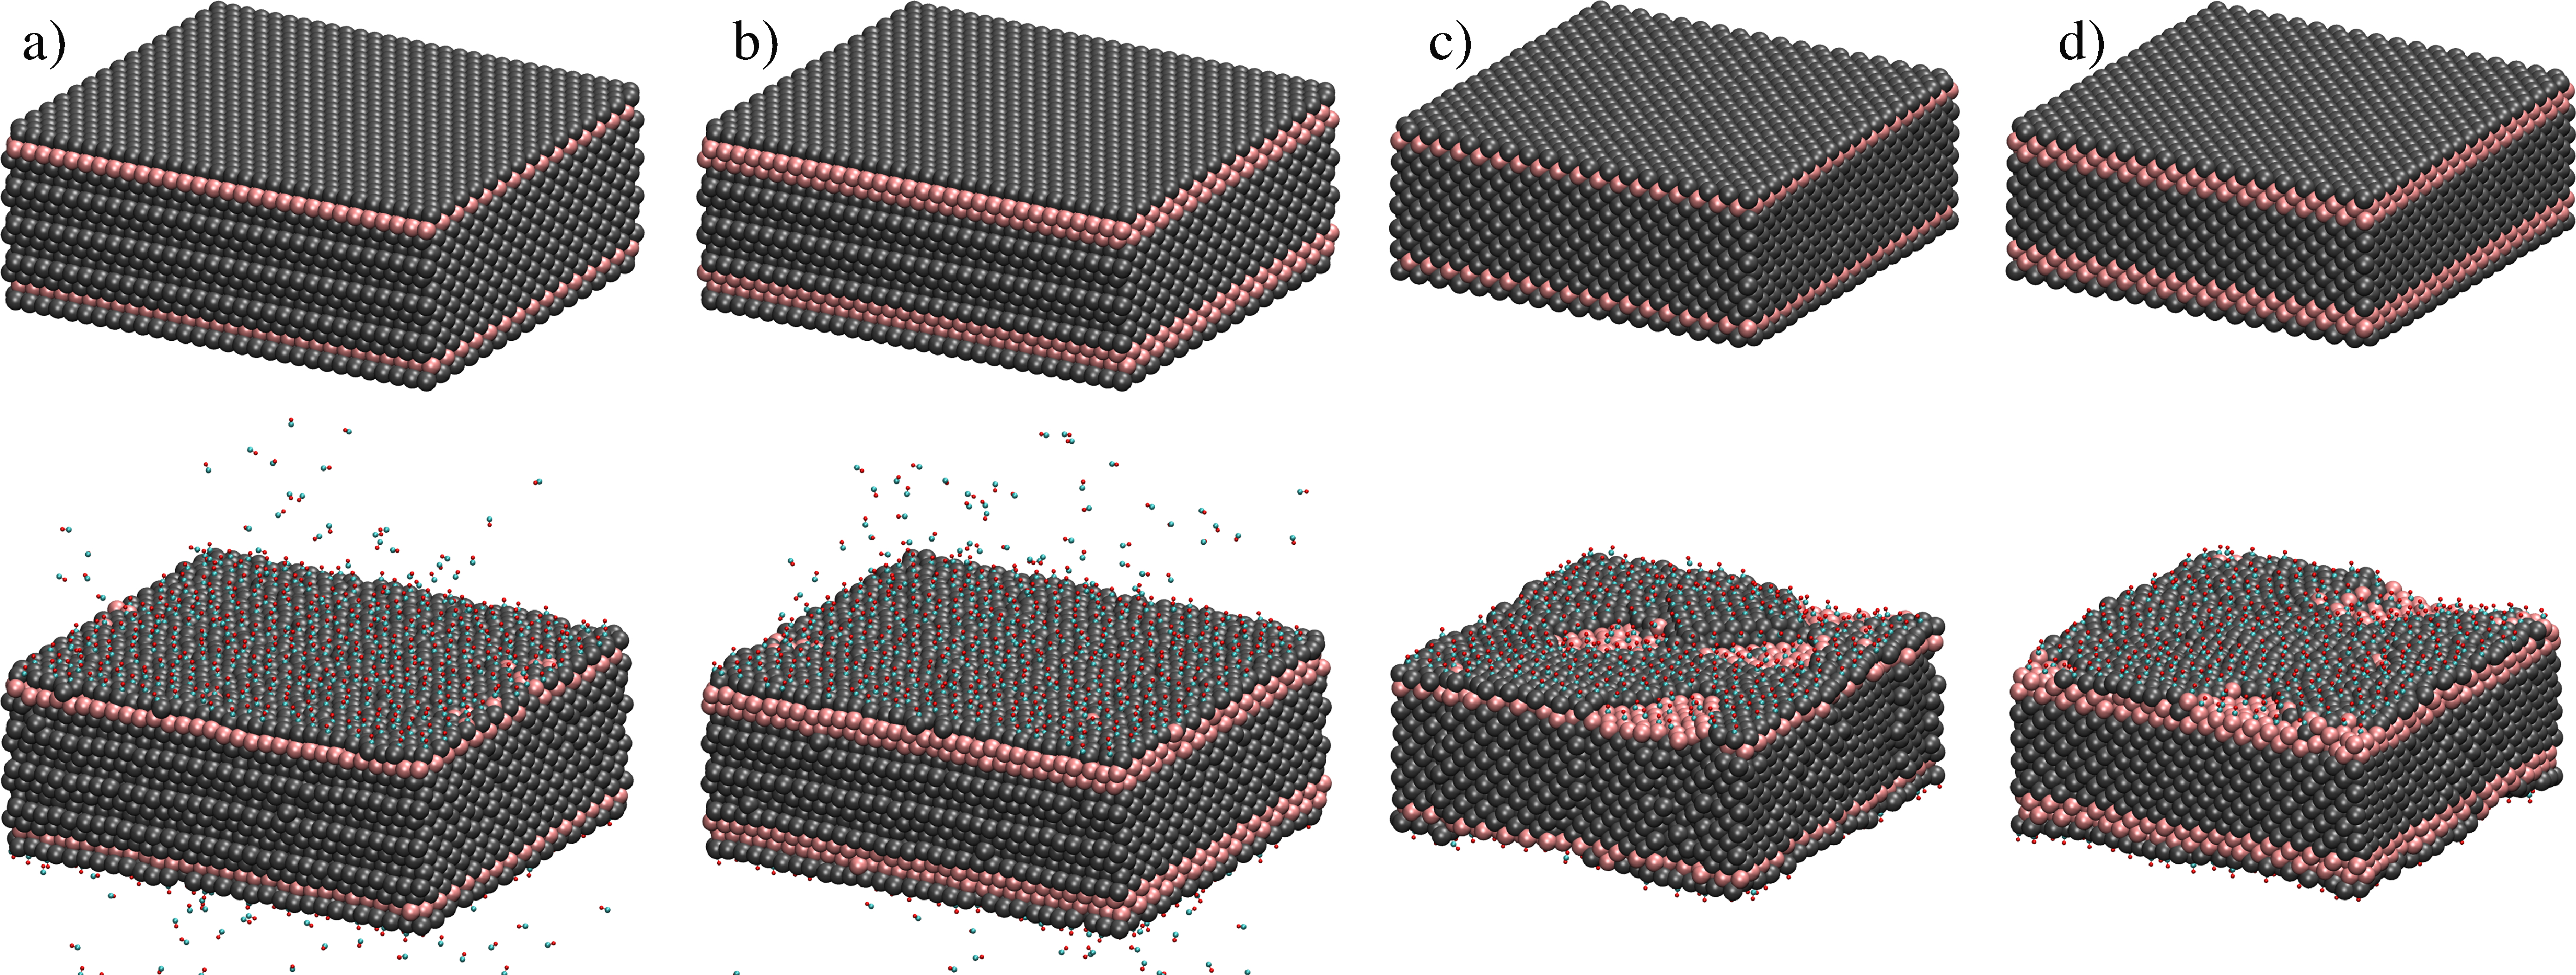
\includegraphics[width=0.8\linewidth]{../figures/appC/systems.pdf}
  \caption{\ce{Pt} atoms are colored gray while \ce{Pd} are colored pink. The
top row depicts near surface alloys with a sandwiched Pt (surface), Pd
(subsurface), Pt (bulk) system before significant warming. Systems (a) and (b)
display the low-energy (111) facets and only differ with number of layers of Pd
with (a) having one layer and (b) having two layers. Systems (c) and (d)
display the (100) facets on the surface and also are only different with regard
to the number of Pd layers, one and two respectively.}
\label{fig:biSystems}
\end{figure}
\end{landscape}

\subsection{System Details}
The systems were constructed from a FCC \ce{Pt} crystal that was ``sliced'' to
display either a (111) or (100) facet in the {\em z}-direction while being
periodic in the {\em x} and {\em y} directions. The bulk of the crystal was
kept as \ce{Pt} while one or two layers directly underneath the surface were
converted to \ce{Pd}. The ideal systems are highlighted in the top row of
Figure \ref{fig:biSystems}. The (111) systems have dimensions of $71.41\times82.44\times100$ while the (100) systems are $68.78\times68.78\times100$.

After warming for ? the systems were dosed with enough Carbon Monoxide (CO) to correspond to 0, 0.25, or 0.5 monolayers (ML) of coverage.




\section{Results \& Discussion}

\subsection{CO-Induced Reconstruction}

\section{Summary}
